\documentclass{article}

\usepackage[final]{neurips_2025}
\usepackage[utf8]{inputenc} % allow utf-8 input
\usepackage[T1]{fontenc}    % use 8-bit T1 fonts
\usepackage{hyperref}       % hyperlinks
\usepackage{url}            % simple URL typesetting
\usepackage{booktabs}       % professional-quality tables
\usepackage{amsfonts}       % blackboard math symbols
\usepackage{nicefrac}       % compact symbols for 1/2, etc.
\usepackage{microtype}      % microtypography
\usepackage{xcolor}         % colors
\usepackage{graphicx}
\usepackage{float}
\usepackage{caption}
\usepackage{subcaption}


\title{Performance Optimization of a Convolutional Neural Network for Real-Time Pulse Detection}

\author{
  Duncan Boyd, Bailey Boyd\thanks{See appendix A. I like using 'we' on formal papers.} \\
  86101888 \\
  \texttt{duncan@wapta.ca} \\
}


\begin{document}


\maketitle


\begin{abstract}
  During CPR, automatically detecting pulse can save precious seconds compared to manual palpation. While devices exist for pulse detection \footnote{For example, my capstone group's device. Note that although it was inspired by it, this work was NOT done as part of my capstone project, which used another algorithm.}, there are limited options when it comes to rigourous detection algorithms. This paper will explore convolutional neural networks (CNNs) as an option for the real-time binary classification of a pulse reading. Using a pulse wave dataset, we swept several critical hyperparameters, optimizing for accuracy. Our final model has achieved an accuracy of [TODO]\%, indicating that the use of CNNs for pulse classification is viable for real-time detection.
\end{abstract}

\section{Introduction}

Cardiopulmonary resuscitation (CPR) is one of the key interventions in cases of cardiac arrest. One of the critical steps during CPR is checking for the return of spontaneous cardiac activity by manually palpating the patient's pulse. Pulse check pauses greater than 10 seconds, the current limit recommended by the Canadian Heart and Stroke Foundation, are associated with increased mortality and morbidity [1]. The purpose of this project is to explore a real time algorithm for pulse detection during CPR. Our goal is to develop an algorithm that is superior to manual palpation (~90\% accurate [2]). This project documents the development and tuning of a 1D CNN that can beat manual palpation in the detection of the pulse in real time.

\section{Input Data}

\subsection{Dataset Description}

The dataset used for this work was collected as part of UBC ECE Capstone Group LS-15's project. It is a series of four second segments, each a time series of pulse data described as sensor values (arbitrary units). Data is sampled at 60Hz, meaning each sample is 240 points in length. A typical sample might look like the plot as shown in figure~\ref{fig:data_example}.

\begin{figure}[H]
    \centering
    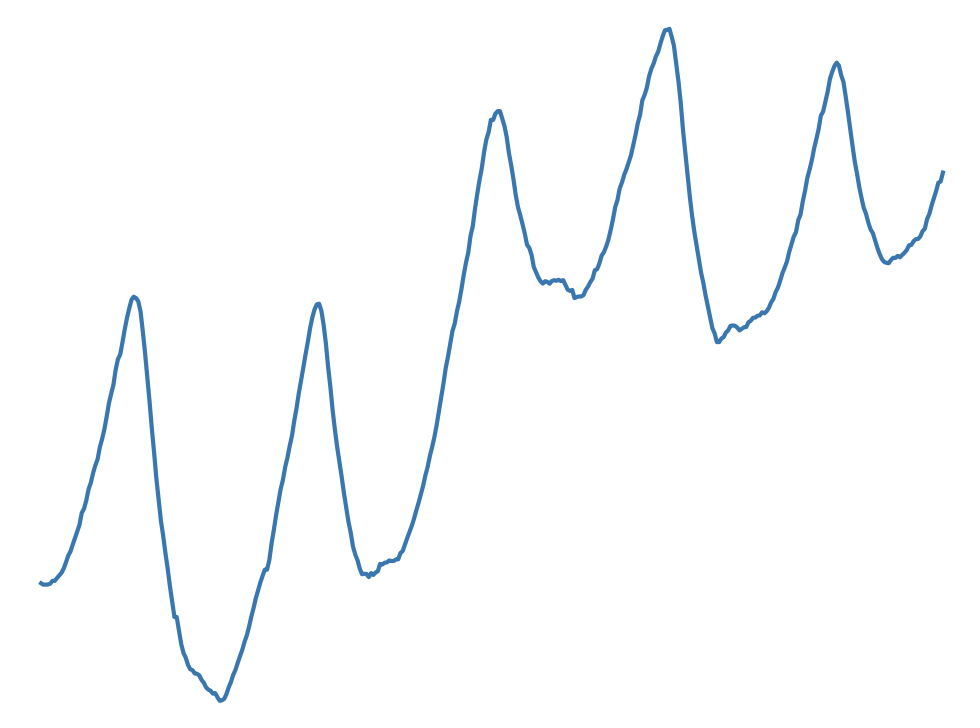
\includegraphics[width=0.5\textwidth]{../media/raw_pulse.png}
    \caption{Typical pulse sample}
    \label{fig:data_example}
\end{figure}

Each data point (four second segment) is labelled by hand as either having, or not having a pulse. The sample in figure~\ref{fig:data_example} would be labelled as having a pulse. Labelling was performed by non-experts, and as such is expected to have some error.

The dataset comprises of 701 data points, collected in a variety of test conditions. The distribution of the data is shown in figure \ref{fig:pulse_distro}. 61\% of data has a pulse, while 39\% does not.

\begin{figure}[H]
    \centering
    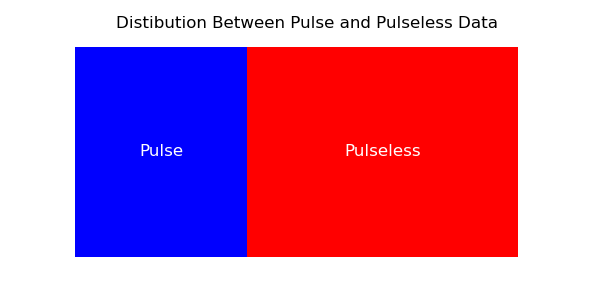
\includegraphics[width=0.5\textwidth]{../media/pulse_bar.png}
    \caption{Dataset distribution}
    \label{fig:pulse_distro}
\end{figure}

Although many samples such as figure~\ref{fig:data_example} may have an easily visible pulse, some samples are more challenging, with spikes created by noise or weak pulse signals. 


\subsection{Preprocessing}

As seen in figure~\ref{fig:data_example}, data often has high and low frequency noise that we would like to filter. After flooring the data by setting the lowest value to 0, we apply a band pass filter as seen in figure~\ref{fig:bpf}. This passes frequencies from 0.5Hz to 5Hz, which translates to 30 BPM and 300 BPM, considered the possible range for the human heart rate.

\begin{figure}[H]
    \centering
    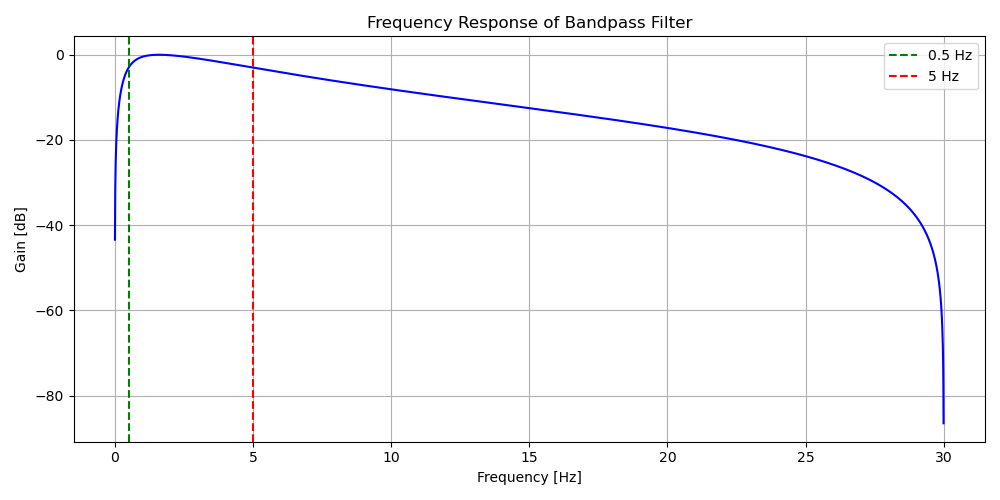
\includegraphics[width=0.8\textwidth]{../media/bpf.png}
    \caption{Frequency response of band pass filter}
    \label{fig:bpf}
\end{figure}

Data often has a strong baseline shift. To eliminate this, we fit a 4th degree polynomial to the data, and then remove that, treating it as a baseline. An example of a fitted polynomial can be found in figure~\ref{fig:poly}

\begin{figure}[H]
    \centering
    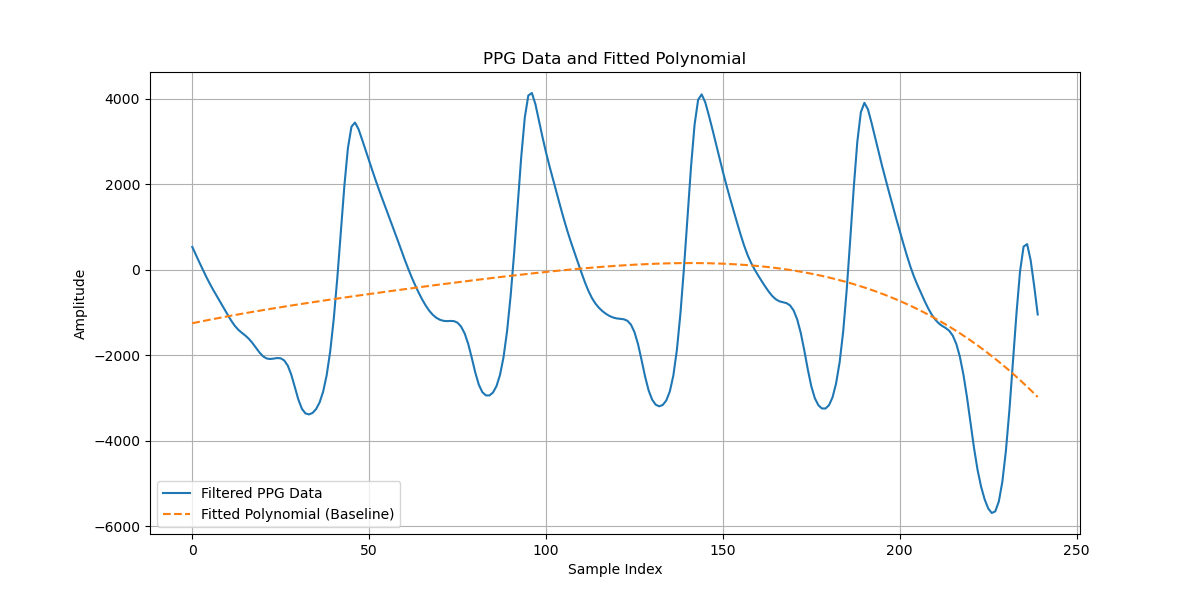
\includegraphics[width=0.8\textwidth]{../media/poly.png}
    \caption{Polynomial fit to data sample}
    \label{fig:poly}
\end{figure}

Finally, data is normalized. The full process makes our data more uniform, allowing for our CNN to focus on features that differentiate pulse.

\begin{figure}[H]
    \centering
    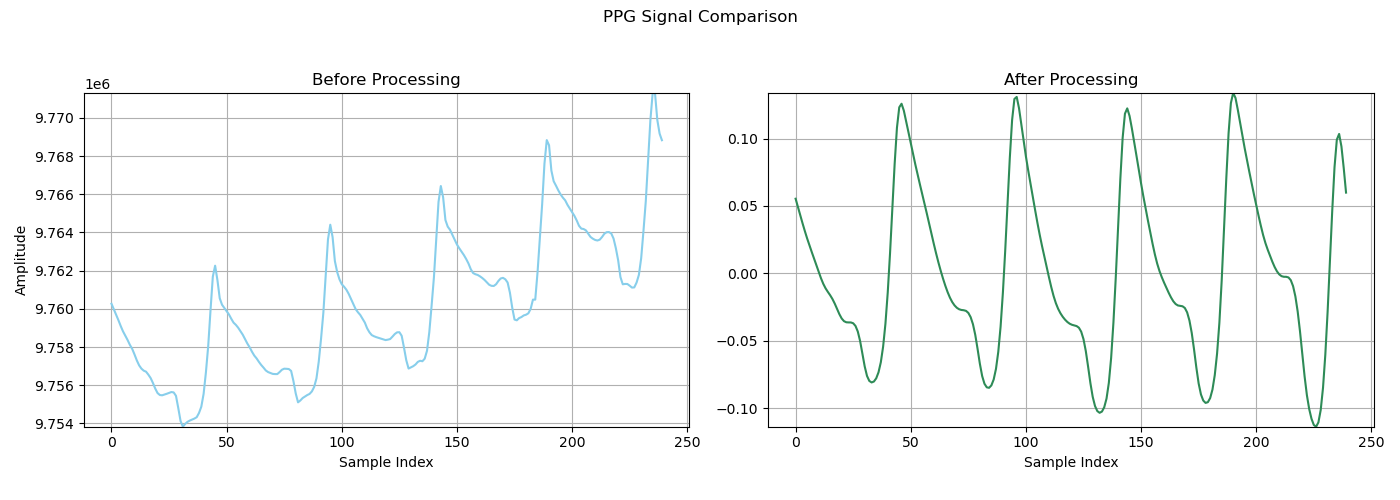
\includegraphics[width=1.0\textwidth]{../media/bef_n_aft.png}
    \caption{Before and after data preprocessing}
    \label{fig:bef_n_aft}
\end{figure}

Although this preprocessing can radically change data points, this results in clean data that performs well in our classification model.

Finally, when data is loaded for model training, it is shuffled randomly to mix up different sections of the dataset.


\section{Model Structure}

To classify four second signals into either a pulse or pulseless category, a 1D CNN was chosen. 1D CNNs are suitable for real time pulse detection because of their efficient feature extraction, resistance to noise, and potential for deployment on a compact architecture. These advantages come at the cost of needing a large, diverse dataset to avoid overfitting.

A typical 1D CNN structure was used, with convolutional layers followed by pooling layers followed by dense layers. A dropout layer was added to test the effectiveness of setting some inputs to zero. As seen in figure~\ref{fig:model}, the number of convolutional and max pooling layers is dependant on the hyperparameter N.

\begin{figure}[H]
    \centering
    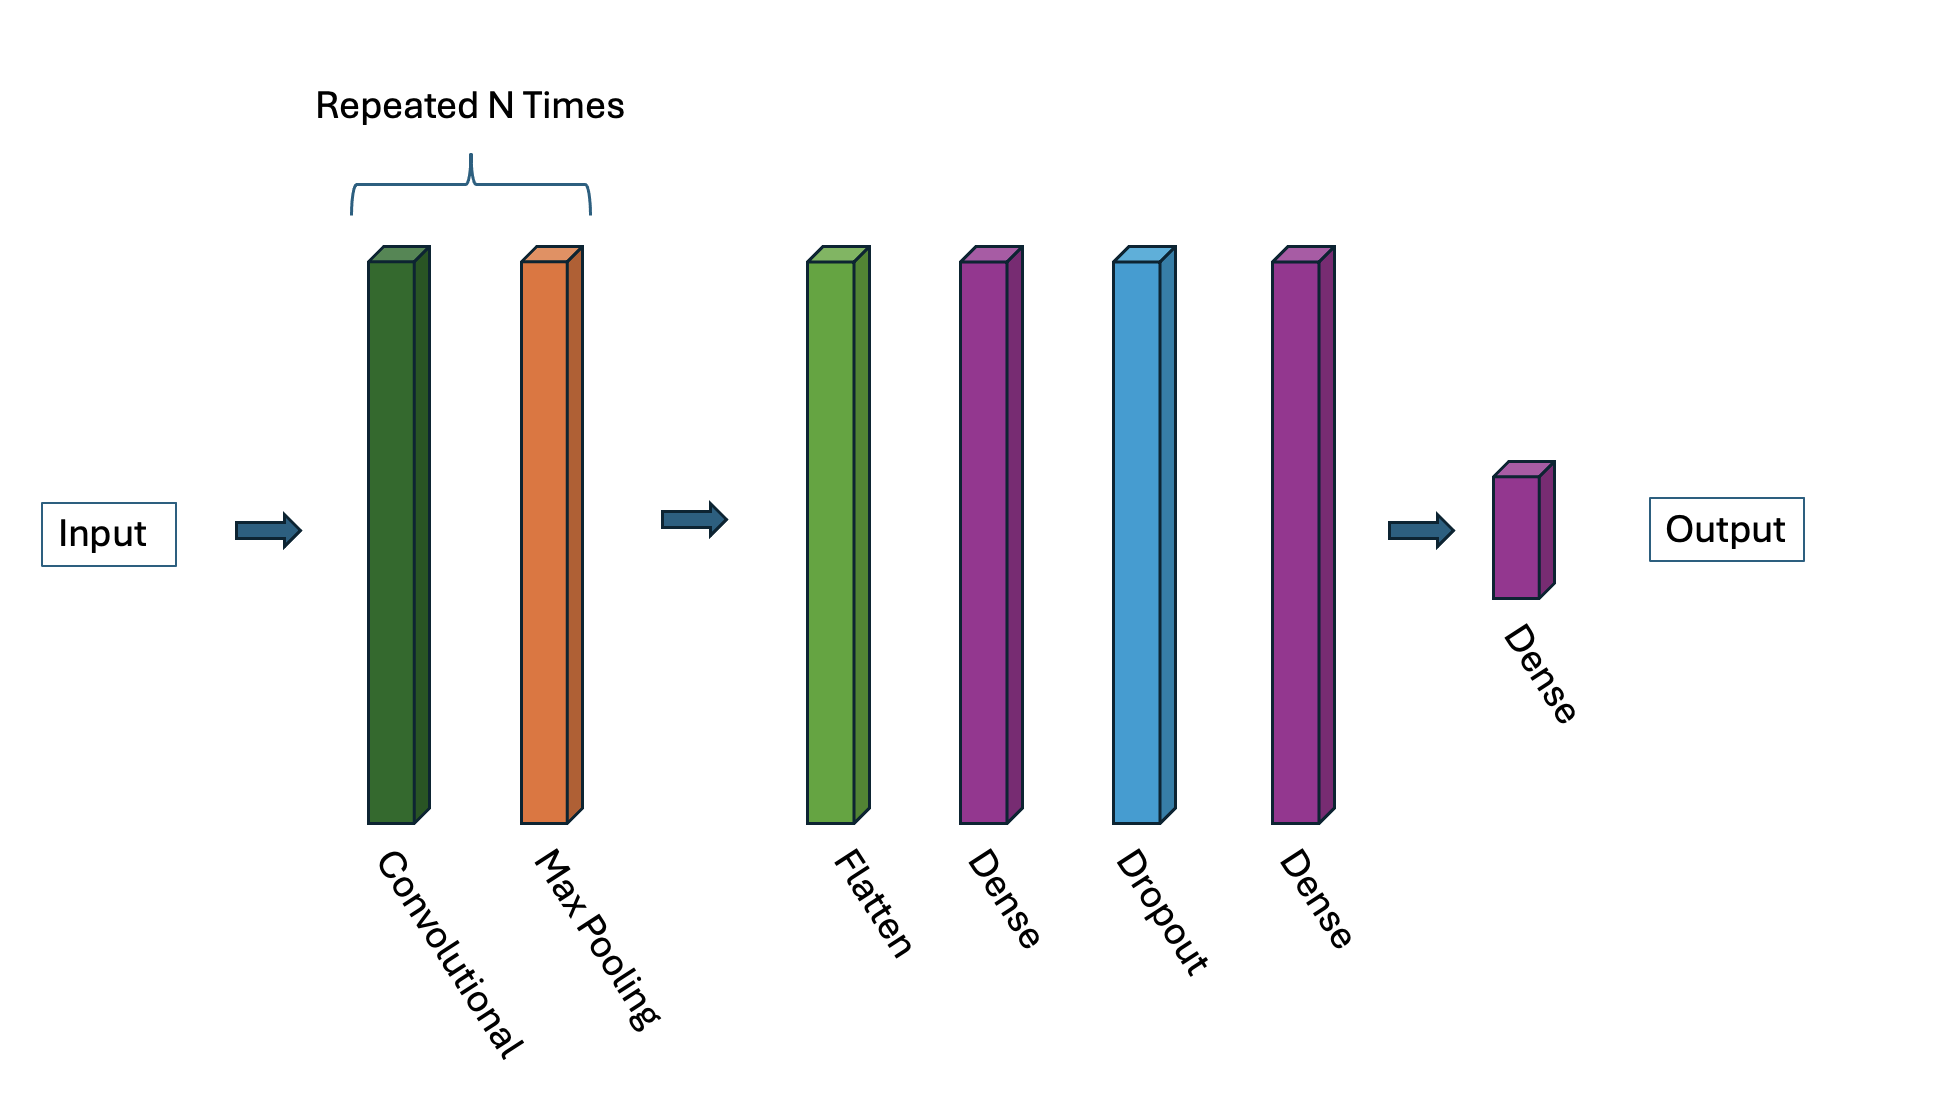
\includegraphics[width=1.0\textwidth]{../media/model.png}
    \caption{Structure of 1D CNN}
    \label{fig:model}
\end{figure}


\section{Model Training} \label{training}

Training was performed using a desktop PC equiped with a Nvidia 1660 Super GPU. Because of limited compatibility with software designed to take advantage of this hardware,  Tensorflow 2.0 was used. Several steps were taken to train and evaluate this model accurately, especially considering the small dataset.


\subsection{Data Augmentation}

The dataset used is collected on few people, and includes only heartrates within a narrow range of possible values. To compensate for this, data augementation was used. The total size of the training dataset was doubled, raising it from 630 data points to 1260. For each sample, a variation was created with an amplitude and a timescale scaled by a random factor.

\begin{figure}[H]
    \centering
    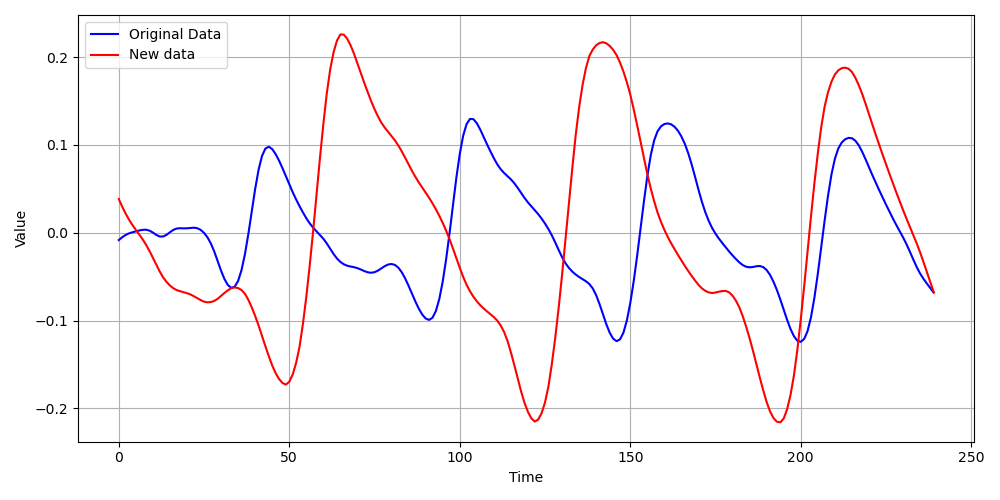
\includegraphics[width=0.8\textwidth]{../media/aug.png}
    \caption{Example of augmented data}
    \label{fig:augmentation}
\end{figure}


\subsection{Data Splitting}

Data is split into a training, test, and validation set. This results in a training set of 1008 points (augmented), a validation set of 252 points (augemented), and a test set of 71 points (not augmented). To mitigate large variations in results due to the small test set, 10 fold training was used. This means that the data was seperated into 10 random train test splits, then trained on each of these models. 

\subsection{Evaluation}

For each set of hyperparameters that we want to test, 10 models are trained using 10 different data splits. The accuracies of these 10 models are averaged to get the accuracy for a given set of hyperparameters.

Models are trained with the Adam optimizer and binary crossentropy loss, common choices for this type of model. Models are trained for a maximum of 200 epochs, but training will be stopped early if no improvements to loss are seen after 5 epochs.


\section{Hyperparameter Sweeps}

Four hyperparameters were targetted for sweeping, convolutional layers, dense points, dropout rate, and L2 rate. See the sections below for more details about these parameters.

When sweeping a parameter, the remaining parameters were set to the following values. These default values were established during preliminary sweeps.

\begin{table}[H]
    \caption{Default parameters}
    \label{parameters}
    \centering
    \begin{tabular}{lll}
      \toprule
      Parameter     & Value  \\
      \midrule
      Convolutional Layers & 3     \\
      Dense Points     & 128     \\
      Dropout Rate     & 0.2  \\
      L2 Rate     & 0.06  \\
      \bottomrule
    \end{tabular}
  \end{table}

Sweeps were evaluated based on the accuracy of each model, as determined in section~\ref{training} above. 


\subsection{Convolutional Layers}

The number of convolutional layers is varied by adding N convolutional layers to the model, each followed by a max pooling layer (see figure~\ref{fig:model}). The number of filter of each subsequent convolutional layer is doubled, starting from 64 filters. This means that a model with N = 3 would have three convolutional layers with 64, 128, and 256 filters each.

The number of convolutional layers was swept from N = 1 to N = 6. The results of this sweep showed that having more layers was generally better. The best performing model used four layers for an accuracy of 95\%. 

\begin{figure}[H]
    \centering
    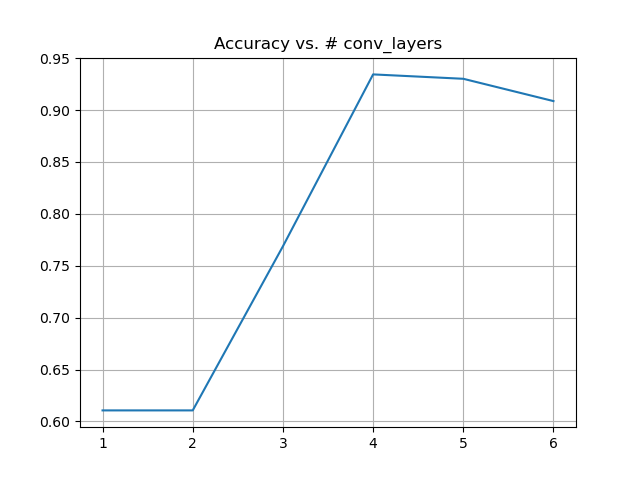
\includegraphics[width=0.8\textwidth]{../media/conv_layers_sweep.png}
    \caption{Convolutional Layers Sweep Results}
    \label{fig:conv}
\end{figure}


\subsection{Dense Points}

The number of dense points in the first two dense layers was swept. A ratio of 2:1 was maintained between the first and second layer  while the number of dense points was swept from 32 to 2042, incrementing in powers of two. This means when testing 256 points, the second dense layer has 256 points while the first has 512 points. 

Surprisingly, the results of this sweep showed that having fewer dense points was generally better. This may be due to overfitting with more dense points. The best performing model used 32 and 64 dense points for an accuracy of 93\%. 

\begin{figure}[H]
    \centering
    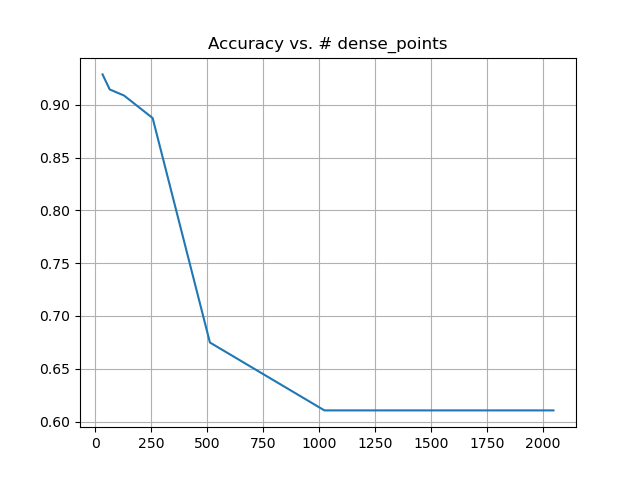
\includegraphics[width=0.8\textwidth]{../media/dense_points_sweep.png}
    \caption{Dense Points Sweep Results}
    \label{fig:dense}
\end{figure}


\subsection{Dropout Rate}

Dropout rate was varied in the dropout layer (see figure~\ref{fig:model}). The rate was varied from 0 to 0.5 with 0.01 increments. The results have little trend for this parameter, with small variance in accuracy compared to previous parameters. The best dropout rate was found to be 0.44, with an accuracy of 93\%.

\begin{figure}[H]
    \centering
    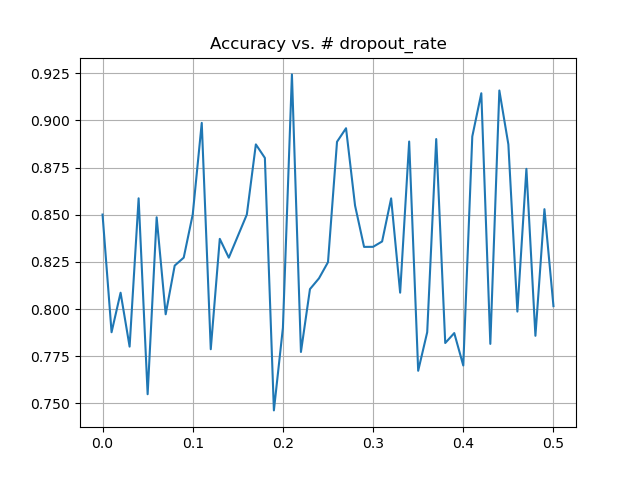
\includegraphics[width=0.8\textwidth]{../media/dropout_rate_sweep.png}
    \caption{Dropout Rate Sweep Results}
    \label{fig:dropout}
\end{figure}


\subsection{L2 Rate}

L2 decay rate was used in the first two dropout layers. The rate was varied from 0 to 0.1 with increments of 0.005. It seems that a lower L2 rate leads to higher and more consistent accuracy. The best L2 rate was found to be 0.045, with an accuracy of 93\%.

\begin{figure}[H]
    \centering
    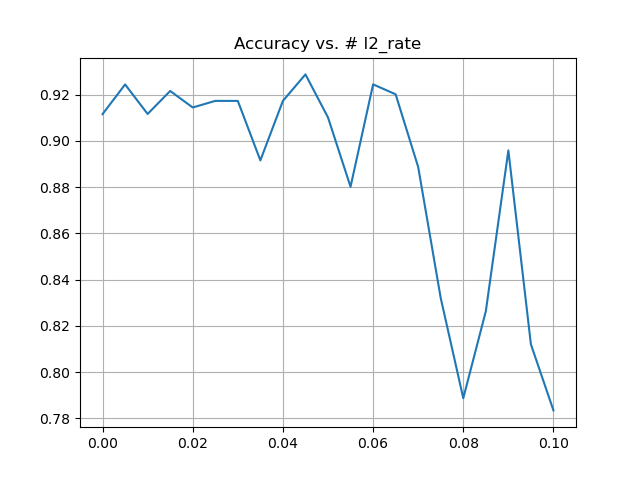
\includegraphics[width=0.8\textwidth]{../media/l2_rate_sweep.png}
    \caption{L2 Rate Sweep Results}
    \label{fig:l2}
\end{figure}


\section{Results}

The hyperparameters as determined by the hyperparameter sweeps are shown in the table below. 

\begin{table}[H]
    \caption{Optimal parameters}
    \label{results}
    \centering
    \begin{tabular}{lll}
      \toprule
      Parameter     & Value  \\
      \midrule
      Convolutional Layers & 4     \\
      Dense Points     & 32     \\
      Dropout Rate     & 0.44  \\
      L2 Rate     & 0.045  \\
      \bottomrule
    \end{tabular}
  \end{table}

After training a model with these parameters, the final model has an accuracy of 96\%. This exceeds any of the accuracies achieved on the parameter sweeps, indicating that this combination is effective.

Some examples of pulse data and the predictions of this model are displayed in the figures below.

\begin{figure}[H]
    \centering
    \begin{subcaptionbox}{Pulse Data\label{fig:image1}}[0.48\textwidth]
        {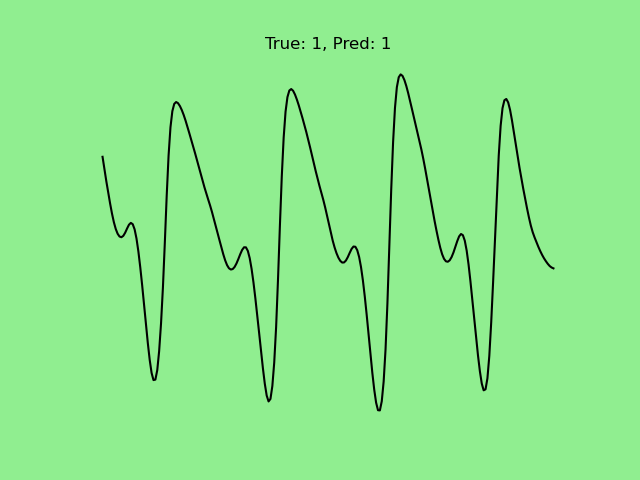
\includegraphics[width=\linewidth]{../media/pulse_1.png}}
    \end{subcaptionbox}
    \hfill
    \begin{subcaptionbox}{Pulseless Data\label{fig:image2}}[0.48\textwidth]
        {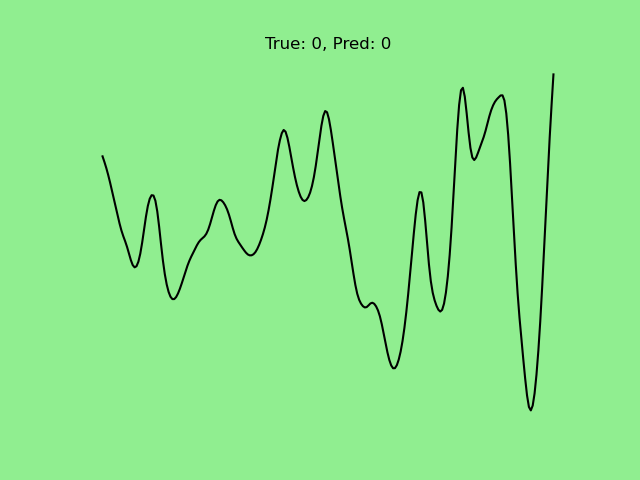
\includegraphics[width=\linewidth]{../media/no_pulse_1.png}}
    \end{subcaptionbox}
    \caption{Correct predictions}
    \label{fig:side_by_side}
\end{figure}

\begin{figure}[H]
    \centering
    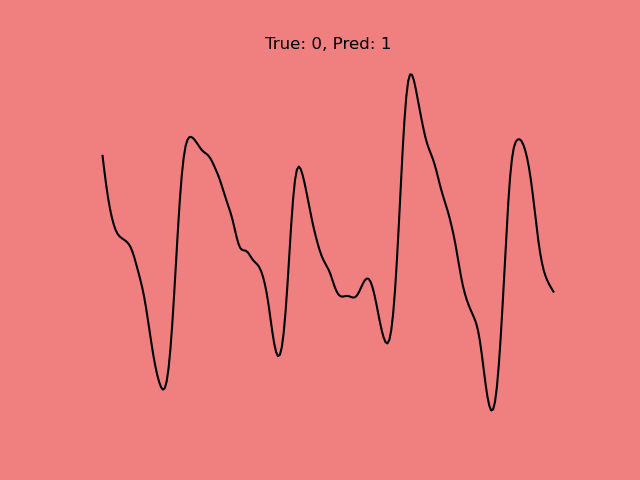
\includegraphics[width=0.5\textwidth]{../media/wrong_2.png}
    \caption{Incorrect prediction}
    \label{fig:wrongo}
\end{figure}

As seen from figure~\ref{fig:wrongo}, the data sample may actually have been labelled incorrectly, but identified correctly by this machine learning model. Many incorrect guesses seem to be on samples that from a human perspective may or may not have a pulse.


\section{Discussion}

These results seem extremely promising, with an accuracy that far exceeds many conventional pulse detection methods . This seems to be a suitable model to implement in a setting where real-time pulse detection is needed and limited data is available. 

There are however some limitations that need to be investigated:
\begin{itemize}

    \item This model is likely overfit, as the dataset it is trained on includes data from few people and at only a narrow range of possible heart rates. Training and testing this archetecture on a larger, more diverse dataset would greatly improve its practical use.
    \item If the hyperparameters are interdependant, the hyperparameters could be further refined with more sweeps. Although gains may be incrementally smaller, this could likely improve the accuracy somewhat. 
    \item Further hyperparameters may have an effect on the model and should be investigated. Optimization of this model still has a lot of potential, as only four parameters were investigated.
    
\end{itemize}

Despite these limitations, this model has yielded extremely impressive results, especially considering the small and somewhat imperfect dataset. There is much potential in using 1D CNNs for pulse detection.

\newpage
\section*{References}
{
\small

[1]	P. A. Meaney et al.\ “Cardiopulmonary Resuscitation Quality: Improving Cardiac Resuscitation Outcomes Both Inside and Outside the Hospital,”\ Circulation, vol. 128, no. 4, pp. 417–435\ Jul. 2013, doi: 10.1161/CIR.0b013e31829d8654.

[2]	L. M. Cunningham, A. Mattu, R. E. O’Connor, and W. J. Brady, “Cardiopulmonary resuscitation for cardiac arrest: the importance of uninterrupted chest compressions in cardiac arrest resuscitation,” The American Journal of Emergency Medicine, vol. 30, no. 8, pp. 1630–1638, Oct. 2012, doi: 10.1016/j.ajem.2012.02.015.
}

\newpage
\appendix

\section{Co-author}

\begin{figure}[H]
    \centering
    \includegraphics[width=0.8\textwidth]{../media/bailey.JPG}
    \caption{Co-author diligently reviewing results}
    \label{fig:bailey}
\end{figure}

\end{document}

